% !TeX root = ../tfg.tex
% !TeX encoding = utf8

\chapter{Análisis de Datos Topológico}
\label{chapter:tda}

En este capítulo, nos centraremos en conocer el análisis de datos topológico y
en cómo se aplica para el estudio de las CNNs. Con el fin de tratar de dar explicación
a cómo transforman los datos las CNNs, proponemos un \textbf{término de
	regularización topológico}, de forma que trataremos de mejorar las capacidades
del modelo penalizando el entrenamiento en base a su complejidad topológica. Más
concretamente, estudiaremos cómo afecta este término tanto en una transferencia
de conocimiento de la red al completo como en un proceso de \textit{fine-tuning}
donde tan sólo entrenaremos la cabeza clasificatoria.

\section{Análisis de datos topológico}

El \textbf{análisis de datos} es una disciplina en la ciencia de datos que emplea
métodos estadísticos, aprendizaje automático y sistemas de procesamiento para
transformar grandes cantidades de datos en información útil para tomar
decisiones en diversos campos \cite{judd2017data}. Con el desarrollo de esta área,
se han integrado técnicas avanzadas como la \textbf{topología algebraica}, que
explora propiedades que se mantienen constantes a pesar de las transformaciones
físicas de los objetos, enfocándose en aspectos como la continuidad y la conectividad
más allá de la forma exacta.

Recordemos que dentro de este contexto, la \textbf{homología} (\autoref{chapter:homology})
destaca como una herramienta de la topología algebraica diseñada para detectar y
analizar características como componentes conexas, agujeros y vacíos en
múltiples dimensiones de un espacio. Por otro lado tenemos la \textbf{hipótesis
	de la variedad} \cite{fefferman2013testingmanifoldhypothesis}, la cual postula que
los datos de alta dimensionalidad suelen residir en variedades de baja dimensión
embebidos en ese espacio de mayor dimensión. Este concepto es importante en el
contexto de las CNNs, pues defiende que estas arquitecturas transforman las variedades
subyacentes de los datos a clasificar hasta hacerlos linealmente separables \cite{cohen2020separability}.
Los conjuntos de datos, que a menudo se presentan como nubes de puntos,
representan muestras discretas que podrían sugerir estructuras subyacentes
similares a \textbf{variedades topológicas} \cite{magai2023deep}. Para explorar
estas estructuras sin introducir sesgos en cómo se conectan estos puntos, se considera
una familia de complejos simpliciales (\autoref{chapter:complex}) en función de la
distancia entre puntos denominados \textbf{filtraciones}, dando lugar al cálculo
de su \textbf{homología persistente} (\autoref{chapter:persistent-homology}). Esta
herramienta no solo identifica características topológicas sino también evalúa su
persistencia a lo largo de diversas escalas, lo que ayuda a distinguir entre el
ruido y las estructuras relevantes.

El \textbf{análisis de datos topológico} (TDA) aprovecha estas técnicas en una metodología
que se centra en desentrañar la estructura subyacente de los datos, basándose en
su \enquote{forma} \cite{carlsson2009topology}. Utilizando la homología
persistente como su herramienta principal, el TDA ofrece una forma robusta y detallada
de identificar características topológicas de los datos, permitiendo revelar
patrones y relaciones no evidentes mediante métodos tradicionales. Esta metodología
se ha aplicado con éxito en varios campos, como la neurociencia para analizar la
conectividad cerebral, en genómica para explorar la interacción entre genes y en
ciencia de materiales para estudiar la estructura microscópica de los materiales
\cite{10.3389/frai.2021.667963}.

El proceso de TDA se organiza en tres fases que facilitan el estudio de la homología
persistente de los datos (\autoref{fig:tda-workflow}):

\begin{enumerate}
	\item \textbf{Preparación de datos}: Inicialmente, se asume que los datos
	están dispuestos en un espacio métrico, típicamente el espacio euclídeo $\R^{N}$,
	utilizando normalmente la distancia euclídea. La elección de la distancia es
	un paso importante, pues determinará la manera en la que se relacionan los
	puntos dentro del conjunto de datos.
	
	\item \textbf{Construcción de filtraciones}: Posteriormente, se construye una
	filtración de complejos simpliciales de Vietoris-Rips a partir de un
	intervalo de radios dado. Generalmente, se trabaja con una muestra finita de
	este intervalo.
	
	\item \textbf{Extracción de características topológicas}: Finalmente, se
	emplea la homología persistente para analizar las filtraciones construidas, obteniendo
	descriptores topológicos que revelan la presencia de características como agujeros
	y conexiones en diversas dimensiones. Estos descriptores proporcionan una
	visión detallada de las propiedades topológicas y geométricas de los datos, ayudando
	a distinguir entre rasgos estructurales significativos y el ruido.
\end{enumerate}

\begin{figure}[h]
	\centering
	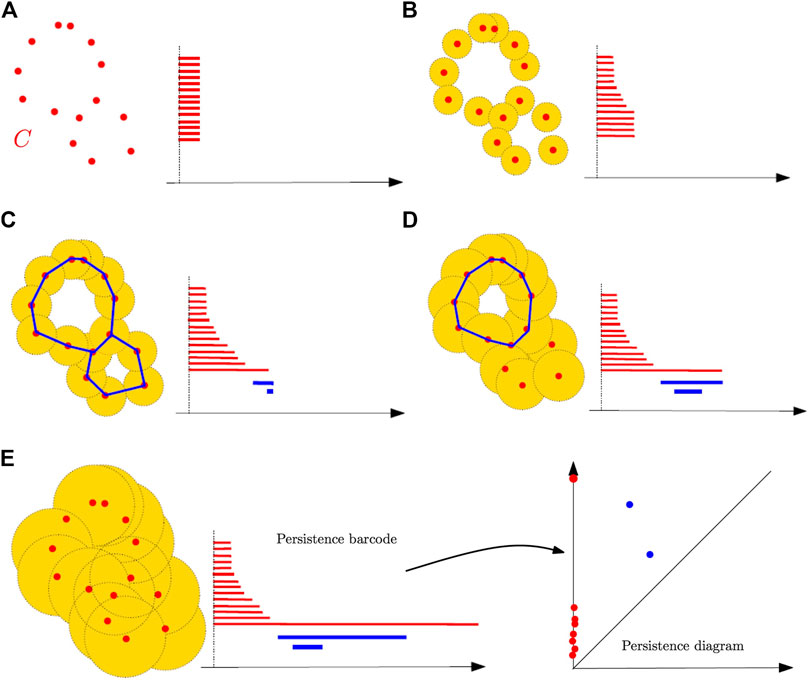
\includegraphics[width=130mm]{img/persistent-homology.jpg}
	\caption{Ejemplo de flujo de trabajo en TDA utilizando complejos de Vietoris-Rips.
		(A) Conjunto inicial de datos. (B,C,D,E) Desarrollo del complejo de Vietoris-Rips
		a distintos niveles de la filtración y el respectivo código de barras hasta
		dicho instante. Finalmente se muestra el diagrama de persistencia resultante,
		mostrando la homología de dimensión 0 (rojo) y de dimensión 1 (azul). Fuente \cite{chazal2021introduction}.}
	\label{fig:tda-workflow}
\end{figure}

\section{TDA en el estudio de CNNs}

Entre las muchas aplicaciones del TDA, nosotros nos centraremos en su uso para el
estudio de las CNNs. Actualmente, existen 3 aproximaciones principales para analizar
estas redes neuronales desde el punto de vista de la topología en función del objeto
de estudio:

\begin{itemize}
	\item \textbf{TDA para el preprocesamiento de imágenes:} Se obtienen diversos
	descriptores topológicos a partir de la imagen a analizar y se estudia cómo
	van cambiando a lo largo de la red. En consecuencia, se proponen
	transformaciones topológicas a las imágenes con el fin de facilitar el
	aprendizaje o la clasificación \cite{garin2019topological}.
	
	\item \textbf{TDA para el análisis de la arquitectura de CNNs:} Se obtiene el
	grafo computacional que define las operaciones de la red y se analiza su
	homología persistente en función de los pesos \cite{chowdhury2018persistent}.
	
	\item \textbf{TDA para el estudio de CNNs en función del conjunto de datos:}
	En esta aproximación, se estudia cómo evoluciona la homología persistente de
	un conjunto de datos a través de las distintas capas de la red. Se aplica
	para comprender cómo las CNNs y sus distintas componentes transforman los
	datos \cite{naitzat2020topology}.
\end{itemize}

En este trabajo, nos centramos en analizar cómo las CNNs modifican los conjuntos
de datos y cómo la \enquote{forma} de los datos influye en su capacidad de
transferencia y clasificación. Naitzat et al. en su artículo \textit{Topology of
	Deep Neural Networks} \cite{naitzat2020topology} exploraron cómo distintas implementaciones
básicas de CNNs, con una tasa de error de generalización inferior al $0.01\%$, alteran
la topología de los datos. En su estudio, realizado sobre conjuntos de datos sintéticos
y reales, concluyeron que estas redes simplifican progresivamente la complejidad
topológica de los datos y que esta simplificación varía según la arquitectura de
la red. Extendiendo este trabajo, German Magai en \cite{magai2023deep} comparó
la homología persistente de varios modelos de aprendizaje profundo en tareas de
clasificación de imágenes utilizando diferentes conjuntos de datos. Magai confirmó
las conclusiones de Naitzat y además señaló que la homología persistente podría servir
como un indicador del error de generalización sin necesidad de conjuntos de prueba.
Adicionalmente, investigaciones como la de Waibel et al. en
\cite{waibel2022capturing} sugieren que la implementación de \textbf{funciones
	de pérdida topológicas} puede mejorar la capacidad de generalización de los modelos
de aprendizaje profundo dadas sus propiedades diferenciables \cite{leygonie2021frameworkdifferentialcalculuspersistence}. %Otra aplicación común en el ámbito del aprendizaje profundo del TDA es la inclusión de \textbf{capas topológicas}, que precisamente tienen en cuenta la topología de los datos para modificarlos en dicho instante \cite{bibid}.% En base a estos hallazgos, nuestro estudio incluirá un término de regularización topológico para tratar de potenciar las capacidades antes mencionadas.

\section{Descriptores topológicos en TDA}

Existen diversas métodos para analizar cómo de compleja es la topología de un conjunto
de datos. En el marco del TDA, el descriptor topológico más sencillo que se puede
obtener es la \textbf{persistencia total}. Dado un código de barras $\mathcal{B}$,
se conoce como persistencia total a la suma de la longitud de los intervalos que
forman el código de barras. Esto es,
\[
TP = \sum_{(b_i,d_i) \in \mathcal{B}}d_{i} - b_{i},
\]
donde $d_{i} \in \R$ denota el instante de muerte de la clase de homología y
$b_{i} \in \R$ el nacimiento de ésta. Pese a su sencillez, la persistencia total
permite estudiar de forma absoluta la homología persistente de un conjunto de
datos en su totalidad.

Otro descriptor comúnmente empleado en el contexto del TDA es la \textbf{entropía
	persistente} \cite{rucco2016characterisation}. Como su nombre indica, este descriptor
calcula la entropía del código de barras respecto a la persistencia total:

\[
PE = - \sum_{(b_i, d_i)\in \mathcal{B}}\frac{d_{i} - b_{i}}{TP}\log\left(\frac{d_{i}
	- b_{i}}{TP}\right).
\]

Más recientemente están empezando a emplearse métodos más sofisticados para
obtener descriptores más informativos. Algunos de ellos buscan lidiar con las clases
de homología con una muerte rápida, pues normalmente son consideradas como
\enquote{ruido}. Por ello, Benjamin Schweinhart \cite{schweinhart2020fractaldimensionpersistenthomology}
presentó la \textbf{dimensión fractal homológica persistente}, que se define como
sigue. Sea $X$ una nube de puntos perteneciente a un espacio métrico y
consideremos $\mathcal{B}_{n}$ como sus códigos de barras de dimensión $n$. Además,
consideremos la suma de potencias de periodos de vida

\[
E_{\alpha}^{n}(X) = \sum_{(d_i, b_i) \in \mathcal{B}_n}(d_{i} - b_{i})^{\alpha}
,
\]

donde $\alpha \geq 0$ es un valor real y $n \in \N$. Dada una medida $\mu$ definida
en $X$, para cada dimensión $n$ definimos la dimensión fractal homológica
persistente $PH\text{dim}_{\alpha}^{n}$ de la medida $\mu$ como:

\[
PH\dim_{\alpha}^{n}(\mu) = \frac{\alpha}{1 - \beta},
\]

donde

\[
\beta = \lim_{m \to \infty}\sup \frac{\log\left(\mathbb{E}\left[ E_{\alpha}^{n}(x_{1},
	\dots, x_{m})\right]\right)}{log(m)},
\]

siendo $x_{1}, \dots, x_{m}$ muestras $\text{i.i.d.}$ de $X$ a partir de la medida
$\mu$ y $\mathbb{E}$ denota la esperanza de dicha variable aleatoria.
Básicamente, este descriptor da más peso a los periodo de vida largos en vez de a
los pequeños, permitiendo que nos centremos en las características topológicas
más relevantes de nuestro conjunto de datos.

\section{Propuesta: regularización con persistencia total normalizada}
\label{subsec:regularizer}

Sin duda, la \enquote{forma} y estructuras que generan los datos en su paso por la
red son características que pueden llegar a ser de gran interés para mejorar diversos
aspectos de un modelo. Con dicha idea en mente, se propone un término de regularización
topológico basado en la persistencia total con el fin de mejorar la capacidad de
clasificación o generalización de la red en función de nuestro interés.

La maximización o minimización de la persistencia total nos permite aumentar o disminuir
la complejidad topológica de nuestros datos respectivamente. Un aumento en la
complejidad topológica implica unos datos más dispersos con estructuras más
complejas, mientras que una minimización de dicha complejidad tiende a agrupar los
datos en estructuras más simples. En el ámbito de las CNNs, el estudio de la persistencia
total a distintos niveles de la red es útil para ver en términos absolutos cómo afectan
los cambios en la red a la homología persistente de los datos \textbf{entre las
	distintas capas}.

En base a lo recién comentado, proponemos el uso de un nuevo descriptor que denominaremos
\textbf{persistencia total normalizada}. A diferencia de la persistencia total,
la persistencia total normalizada calcula el cociente de cada uno de los
intervalos del código de barras respecto a aquel con un mayor ciclo de vida. En caso
de que un ciclo de vida fuese infinito, se truncaría en el último instante de
muerte de una clase de homología persistente previo a él. Este descriptor es una
métrica relativa, de utilidad para estudiar la tendencia \textbf{intracapa} de la
homología persistente que sufren los datos a lo largo de la red.

En consecuencia, para un código de barras $\mathcal{B}$ podemos definir un
término de regularización $\Omega(\mathcal{B})$ que minimice la persistencia de
forma que

\[
\Omega(\mathcal{B}) = \frac{TP}{L}= \frac{1}{L}\cdot \sum_{(b_i,d_i) \in
	\mathcal{B}}d_{i} - b_{i},
\]

donde $L = \max_{(b_i,d_i) \in \mathcal{B}}\{ d_{i} - b_{i} \}$ es el intervalo
de mayor longitud. Nótese que dicho intervalo siempre va a representar el ciclo de
vida de una clase de homología de dimensión 0, pues nacen en el primer instante
y solamente mueren si la cadena que representa se ha fusionado con otra
componente conexa. Luego siempre existe una componente conexa que vive durante toda
la filtración. Además, al aplicar el cociente sobre la longitud del mayor intervalo,
logramos relativizar la complejidad respecto al tamaño de la filtración, lo que nos
proporciona un mayor control.

Por ejemplo, en el caso $\Omega(\mathcal{B}) = 1$ esto implica que tan solo
existe una componente conexa. El término aplicaría de forma que

\[
J_{\Omega}(\mathbf{w}) = J(\mathbf{w}) + \alpha \Omega(\mathcal{B})
\]

siendo $J$ la función objetivo, $\mathbf{w}$ los pesos de la red y
$\alpha \in [-1, 1]$. En el caso donde $\alpha > 0$, estaríamos disminuyendo la
complejidad topológica mientras que un valor $\alpha < 0$ implicaría un aumento
en la complejidad de la topología.

Nuestro objetivo en esta última fase será aplicar el término de regularización
con dos fines distintos. Primero, trataremos de mejorar la capacidad de
clasificación del modelo disminuyendo la complejidad topológica de los datos en
la cabeza clasificatoria. Por último, trataremos de utilizar dicho término para
mejorar la capacidad de transferencia de los modelos. Exploraremos dos vías:
buscaremos mejorar la capacidad de transferencia de un modelo más sencillo (con menos
clases) a uno más general (con más clases) aumentando su persistencia total
normalizada y viceversa disminuyéndola.

\endinput
%--------------------------------------------------------------------
% FIN DEL CAPÍTULO.
%--------------------------------------------------------------------